\section{Para-real method}
	
Para-real method is a parallel-in-time integration methods which was introduced in 2001 by Lions, Maday and Turinici. Parareal computes the numerical solution for multiple time steps in parallel, it is categorized as a parallel across the steps method.

\subsection{Explanation}

As for the previous methods, we consider an initial value problem of the form \\
\begin{minipage}{\linewidth}
	\centering
	$\left\{\begin{aligned}
		X'&=f(t,X) \qquad t_0\le t\le T \\
		X(t_0)&=X_0
	\end{aligned}\right.$ \\
\end{minipage} \\

\noindent Parareal method need a decomposition of the time interval $[t_0,T]$ into $P$ slices $[t_j,t_{j+1}]$ with  $j\in\{0,\dots,P-1\}$ where $P$ is the number of process units. We want to parallelize the algorithm so each time slice is assigned to one process. We denote by $F$ a function which is of high accuracy and $G$ which is of low accuracy. Also, $F$ will be very expensive in terms of calculation but very accurate and $G$ will be very cheap but very imprecise. We denote by $\Delta t_F$ the fine time step and by $\Delta t_G$ th coarse time step. To have the right number of points in total (i.e. the sum of the number of points of each interval is equal to the number of points between $t_0$ and $T$), we are not going to cut the interval in equal parts but the $t_j$ will have to be multiples of $\Delta t_G$ (we will choose the multiple of $\Delta t_G$ closest to $t$ which cuts our interval in equal parts).
For example, taking $P=3$ processes, $\Delta t_G=0.1$ and an interval from $t_0=0$ to $T=2$, our exact $t_j$ will be : $[0,\;0.666,\;1.333,\;2]$ which we will be approximated  by $[0,\;0.7,\;1.3,\;2]$. We will also suppose that the coarse time step $\Delta t_G$ is a multiple of the fine time step $\Delta t_F$. If this was not the case, a simple way to avoid the problems related to the number of points could be an interpolation between the two time steps $\Delta t_F$ closest to $\Delta t_G$. \\

\noindent We denote by $U_j^k$, $j\in\{0,\dots,P\}$ the initial point at time $t_j$ and at iteration k. We also note $F(U_{j-1}^k)$, $j\in\{1,\dots,P\}$ the fine integrator between $t_{j-1}$ and $t_j$ which start by the initial point $U_{j-1}^k$ at iteration k and respectively $G(U_{j-1}^k)$, $j\in\{1,\dots,P\}$ the coarse integrator between $t_{j-1}$ and $t_j$ which start by the initial point $U_{j-1}^k$ at iteration k. Then, a series of steps (\textit{see \ref{parareal}}) is performed until the solution of the system converges. \\

\noindent At iteration $k=0$ :
\begin{enumerate}[label=\textbullet]	
	\item Step 1 (\textit{see \ref{parareal:1}}) : At iteration $k=0$, we have an initial point $U_0^0=X_0$.
	\item Step 2 (\textit{see \ref{parareal:2}}) : We start by applying the function $G$ on all intervals $[t_j,t_{j+1}]$ and we note $U_j^0=G(U_{j-1}^0)$ the values of $G$ at $t_j$. \\
	Note that this part of the method can be done sequentially because if we parallelize the task, the process $j$ should wait until the process $j-1$ has finished before starting.
	\item Step 3 (\textit{see \ref{parareal:3}}) : We can then calculate from each $U_j^0$ the fine solution between $t_j$ and $t_{j+1}$ : $F(U_j^0)$. This is an operation that must be parallelized.
\end{enumerate}

\noindent At iteration $k=1$ :
\begin{enumerate}[label=\textbullet]	
	\item Step 4 (\textit{see \ref{parareal:4}}) : We can then continue to iteration $k=1$ where we need the values $G(U_j^0)$ and $F(U_j^0)$ calculated at the previous iteration ($k=0$). \\
	We will also keep the initial point at time $t_0$ : $U_0^1=U_0^0$.
	\item Step 5 (\textit{see \ref{parareal:5}}) : We can then calculate $G(U_0^1)$ which allows us to obtain the point $U_1^1$ by the following formula:
	$$U_j^1=G(U_{j-1}^1)+(F(U_{j-1}^0)-G(U_{j-1}^0))$$
	Note that due to $U_0^1=U_0^0$, we have $G(U_0^1)=G(U_0^0)$ and therefore $U_1^1=F(U_0^0)$ \\
	We then compute in the same way the following $G(U_j^1)$ and the associated $U_{j+1}^1$ points. This step can be done sequentially for the same reason as in step 2.
	\item Step 6 (\textit{see \ref{parareal:6}}) : We can then calculate from each $U_j^1$ the fine solution between $t_j$ and $t_{j+1}$ : $F(U_j^1)$. This is an operation that must be parallelized. \\
	Note that due to $U_0^1=U_0^0$, we also have $F(U_0^1)=F(U_0^0)$.
\end{enumerate}

\noindent Then we repeat steps 3 to 6 until $U_j^k-U_j^{k-1}\rightarrow 0 \quad \forall j\in\{0,\dots,P-1\}$. We have :
$$U_j^k=G(U_{j-1}^k)+(F(U_{j-1}^{k-1})-G(U_{j-1}^{k-1}))$$

\begin{figure}[h]
	\captionsubfigure
	\fbox{
		\centering \qquad
	\begin{minipage}[c]{\linewidth}
	\begin{subfigure}[t]{.30\linewidth}       
		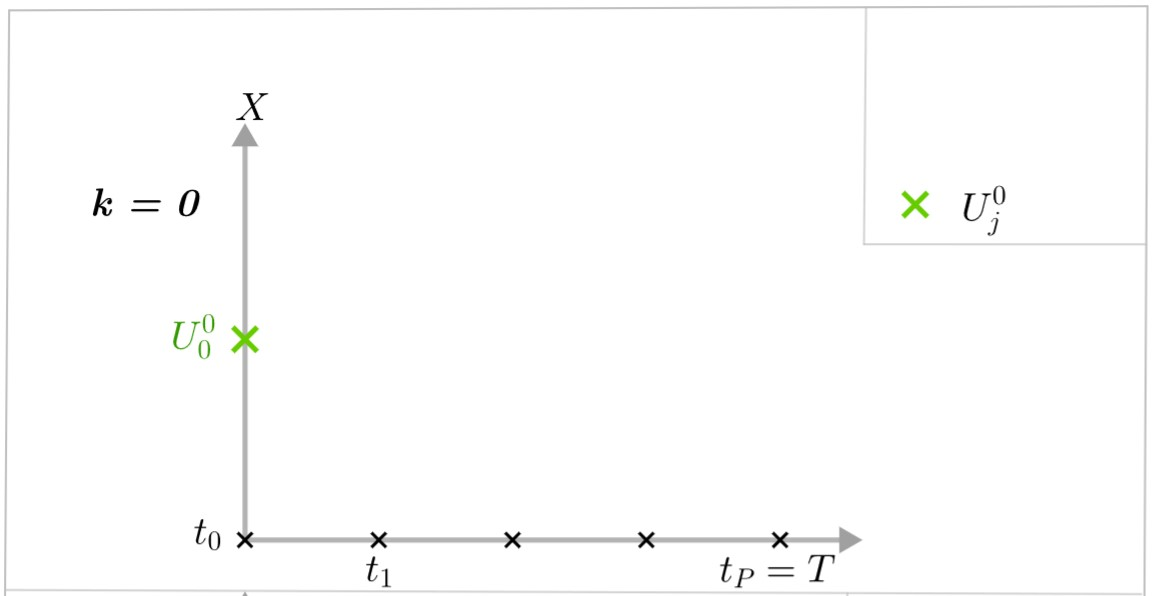
\includegraphics[width=\linewidth]{"images/parareal/parareal_1.jpg"}
		\captionof{figure}{ : Step 1}
		\label{parareal:1}
	\end{subfigure} 
	\begin{subfigure}[t]{.30\linewidth}       
		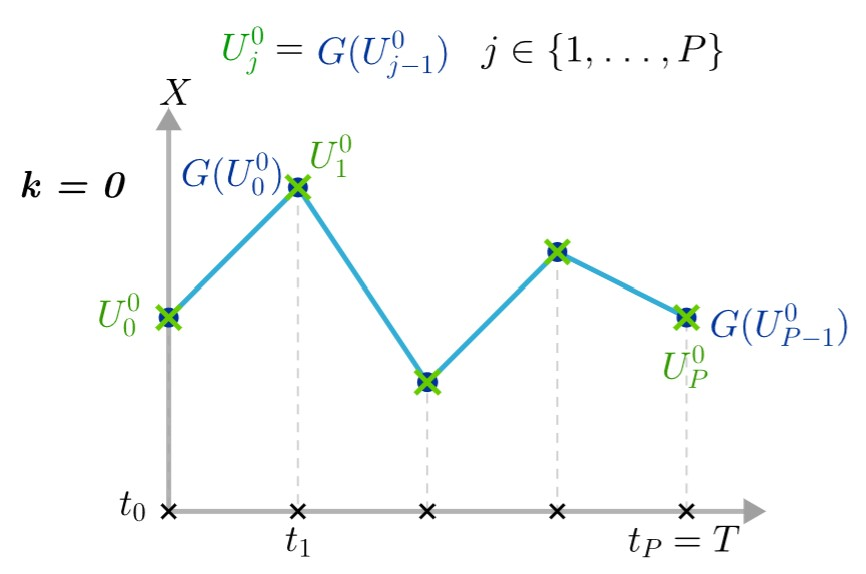
\includegraphics[width=\linewidth]{"images/parareal/parareal_2.jpg"}
		\captionof{figure}{ : Step 2}
		\label{parareal:2}
	\end{subfigure} 
	\begin{subfigure}[t]{.30\linewidth}       
		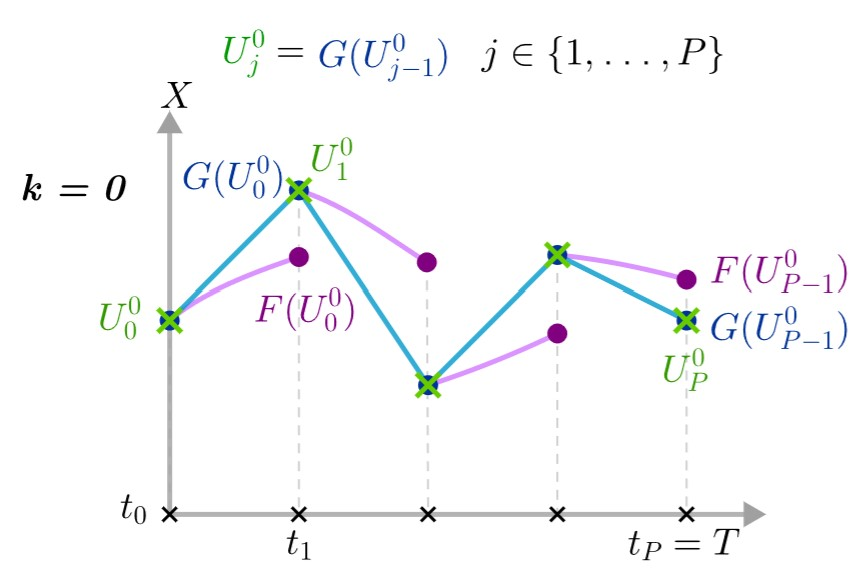
\includegraphics[width=\linewidth]{"images/parareal/parareal_3.jpg"}
		\captionof{figure}{ : Step 3}
		\label{parareal:3}
	\end{subfigure} 
	
	\begin{subfigure}[t]{.30\linewidth}       
		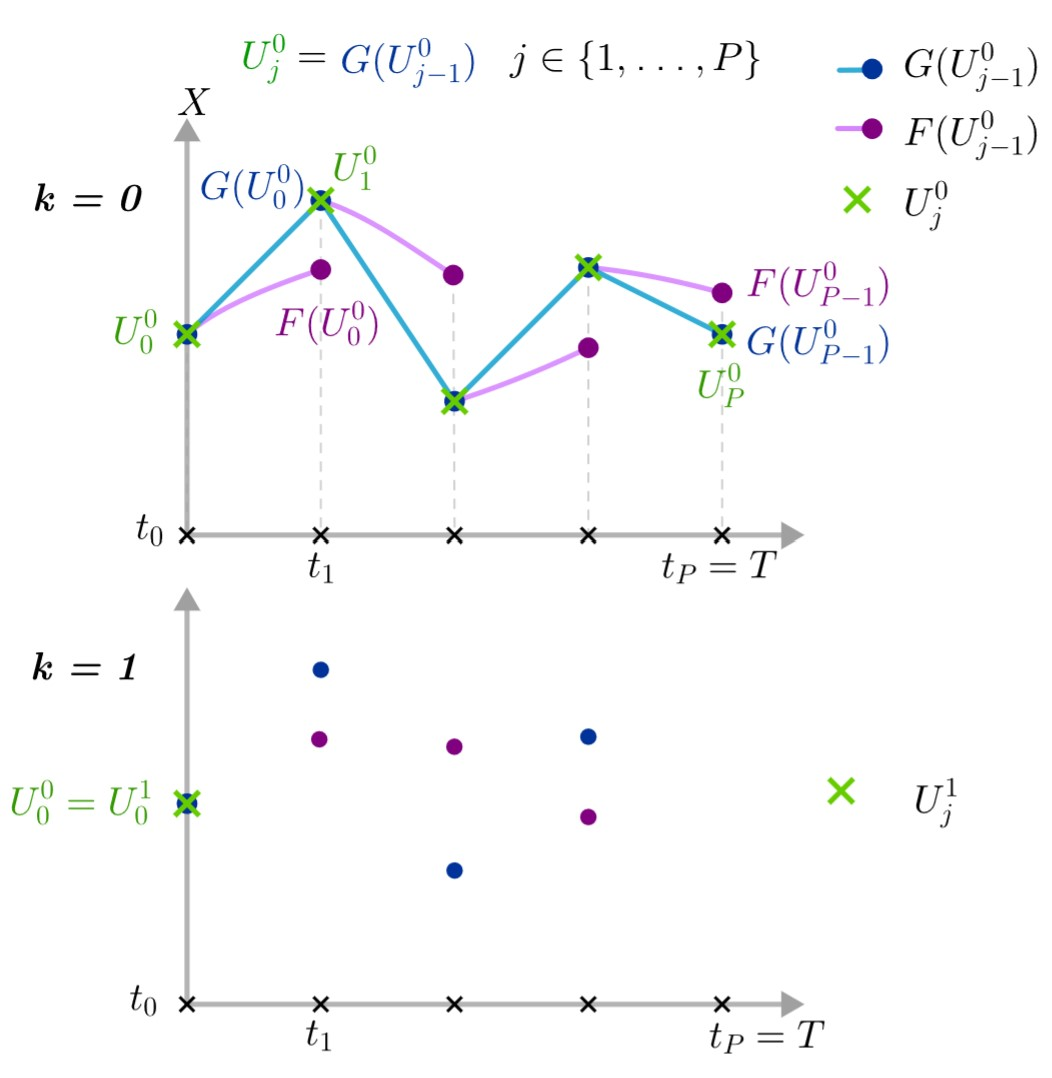
\includegraphics[width=\linewidth]{"images/parareal/parareal_4.jpg"}
		\captionof{figure}{ : Step 4}
		\label{parareal:4}
	\end{subfigure} 
	\begin{subfigure}[t]{.30\linewidth}  
		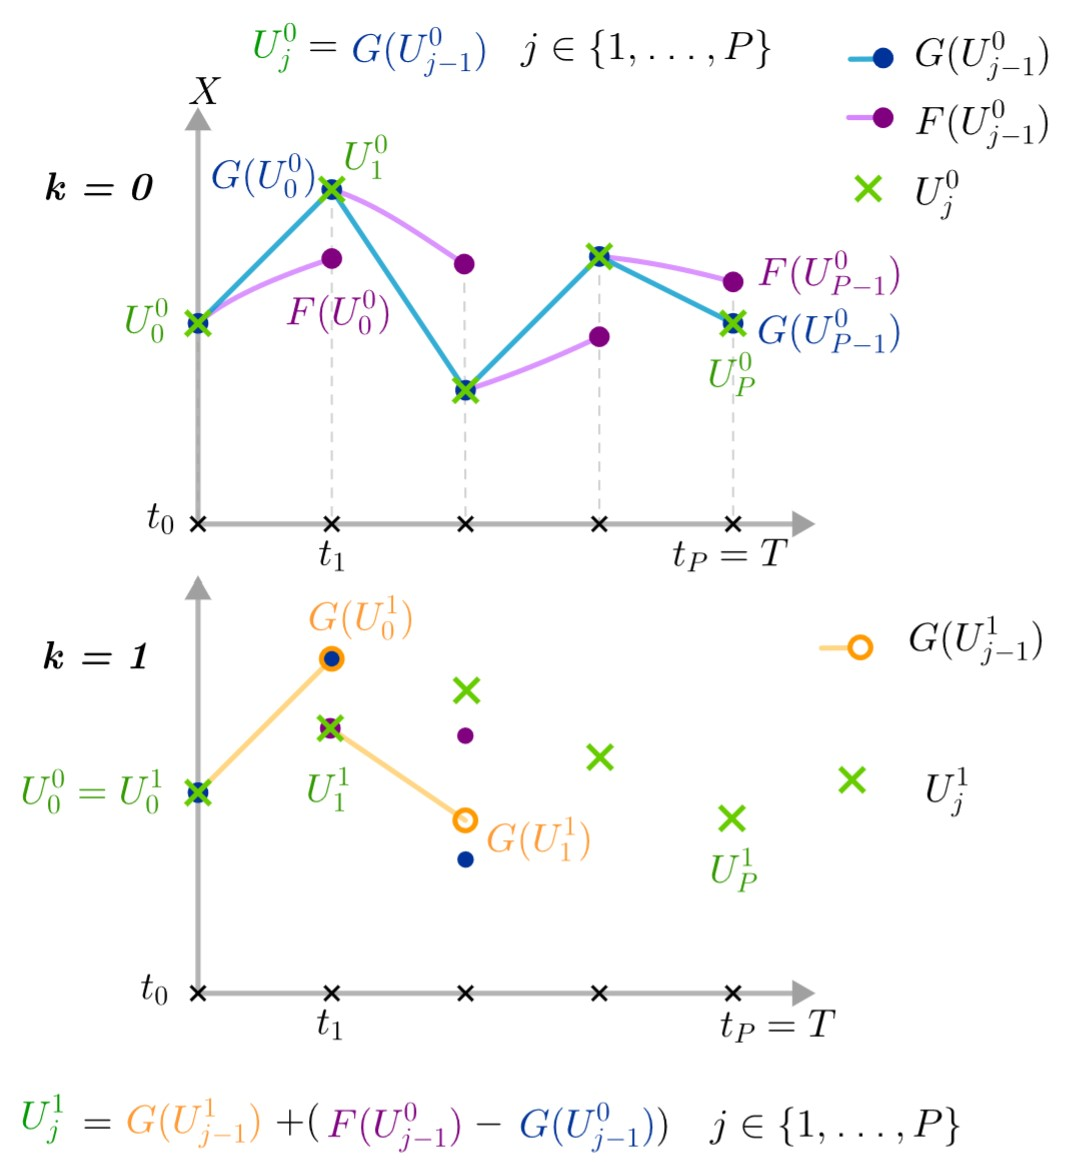
\includegraphics[width=\linewidth]{"images/parareal/parareal_5.jpg"}
		\captionof{figure}{ : Step 5}
		\label{parareal:5}
	\end{subfigure} 
	\begin{subfigure}[t]{.30\linewidth}      
		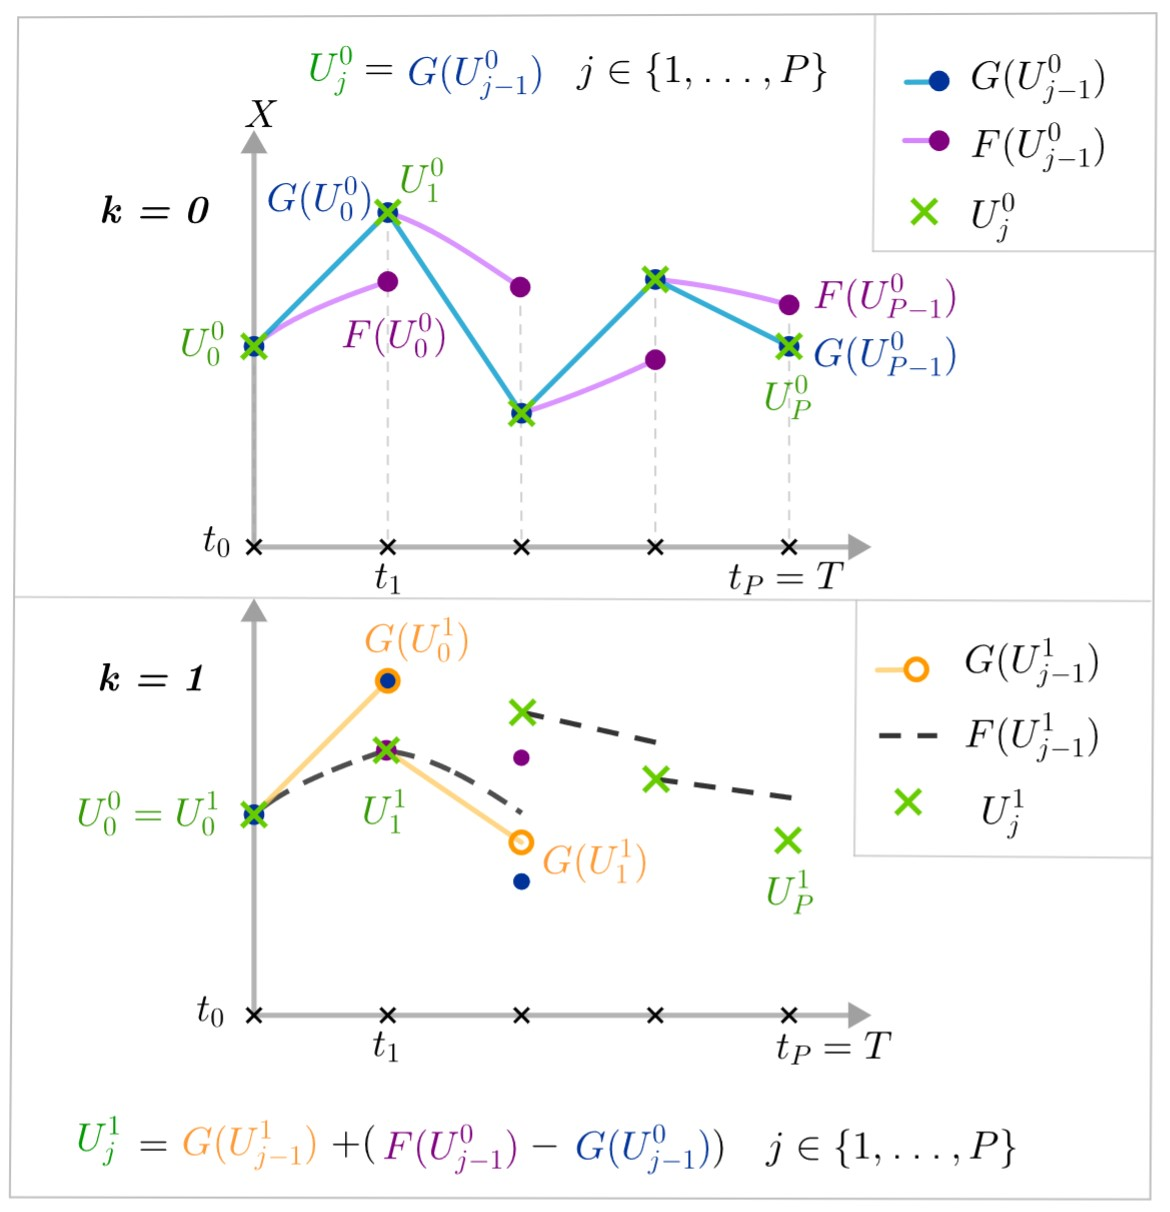
\includegraphics[width=\linewidth]{"images/parareal/parareal_6.jpg"}
		\captionof{figure}{ : Step 6}
		\label{parareal:6}
	\end{subfigure}
	\end{minipage}}
	\caption{Parareal method}
	\label{parareal}
\end{figure}

\newpage

\noindent \underline{\textit{Notes :}} Following k iteration.
\begin{itemize}
	\item We have : $\qquad U_0^k=U_0^0=X_0 \quad \forall k$.
	\item Note that the first 2 steps are always done because there can't be convergence with only one value. So for example if we take only one process and we apply the parareal method, we will have at the first iteration ($k=0$) only one initial point $U_0^0=X_0$ and we will compute the fine and coarse solution only on this point. We can then go to the next iteration which will be exactly the same and the algorithm will stop immediately. Indeed, there will be convergence between $U_0^0$ and $U_0^1$ (because they are equal), moreover there is obviously convergence between the 2 solutions. However, there is still one extra iteration ($k=1$) and the computation of the coarse solution is also useless because it is not used to compute the other initial points due to the fact that there is only one.
	\item We can also notice that the calculations which are done on the last interval $[t_{P-1},t_P]$ are not used because the points $U_P^k$ are not useful for the method. On this interval, one could then compute the fine solution only if there is convergence.
\end{itemize}

\subsection{Application to the harmonic oscillator}

\noindent Before moving on to the Lorenz system, we will consider a mass-spring system of the following form :

\begin{equation}
	\frac{\partial^2 x}{\partial t^2}+\omega_0^2 x = 0 \quad \iff \quad \frac{\partial^2 x}{\partial t^2}=-\omega_0^2 x \quad \text{with} \quad \omega_0=\sqrt{\frac{k}{m}}
	\label{osc}
\end{equation}

\noindent $\omega_0$ is called the natural pulsation of the harmonic oscillator. $k$ and $m$ are the spring stiffness and the suspended mass respectively. We are interested in this equation because its exact solution is known and is of the form :

$$x(t) = x_0 \cos(\omega_{0}t+\phi_0)$$

\noindent First of all, the numerical methods we have seen in Section \ref{sec4} (such as Runge Kutta order 4 in section \ref{sec4.4}), allow us to solve first order differential equations. But the harmonic oscillator equation \ref{osc} is a second order equation. We will therefore start by making a simple change of variable which will allow us to replace this second order differential equation by a system of two first order equations. We pose :
 
$$\qquad \frac{\partial x}{\partial t}=v \quad \Rightarrow \quad \frac{\partial^2 x}{\partial t^2}=\frac{\partial v}{\partial t}$$

\noindent And so the equation becomes :

$$\left\{\;\begin{aligned}
	\frac{\partial x}{\partial t}&=v \\
	\frac{\partial v}{\partial t}&=-\omega_0^2 x
\end{aligned}\right.
$$

\noindent Let's take an example to understand how we can determine the exact solution from the initial conditions that we will take. For example if we take $\omega_0=5$ and $(x(0),v(0))=(0,1)$, we have :

$$\left\{\;\begin{aligned}
	x(0)&=0 \\
	v(0)&=1
\end{aligned}\right. \quad \Rightarrow 
\left\{\;\begin{aligned}
	x_0 \cos(\phi_0)&=0 \\
	-x_0 \omega_{0} \sin(\phi_0)&=1
\end{aligned}\right.  \quad \Rightarrow  
\left\{\;\begin{aligned}
	x_0&=\frac{-1}{5} \\
	\phi_0&=\frac{\pi}{2}
\end{aligned}\right.
$$

\noindent And thus the solutions of the equation are of the form :

$$x(t) = \frac{-1}{5}\cos(5t+\frac{\pi}{2})$$

\noindent We want now to apply the parareal method on the harmonic oscillator. For the two integrators we will take Runge Kutta order 4 method with a little time step for $F$ and a larger one for $G$. \\

\colorbox{yellow}{TO COMPLETE : convergence of the method}

\subsection{Application to the Lorenz system}

We try now to apply this method on the Lorenz system. In the previous explanation, we have also :

$$X'=\begin{pmatrix}
    x' \\
    y' \\
    z'
\end{pmatrix}, \quad X=\begin{pmatrix}
    x \\
    y \\
    z
\end{pmatrix} \quad et \quad f(t,X)=\begin{pmatrix}
    \sigma(y-x) \\
    x(r-z)-y \\
    xy-bz
\end{pmatrix}$$

\noindent For the two integrators we will take Runge Kutta order 4 method with a little time step for $F$ and a larger one for $G$. \\

\colorbox{yellow}{TO COMPLETE : example of result}
